\documentclass[12pt]{report}
\usepackage[utf8]{inputenc}
\usepackage[russian]{babel}
%\usepackage[14pt]{extsizes}
\usepackage{listings}
\usepackage{graphicx}
\usepackage{amsmath,amsfonts,amssymb,amsthm,mathtools} 
\usepackage{pgfplots}
\usepackage{filecontents}
\usepackage{indentfirst}
\usepackage{eucal}
\usepackage{amsmath}
\usepackage{enumitem}
\frenchspacing

\usepackage{indentfirst} % Красная строка


%\usetikzlibrary{datavisualization}
%\usetikzlibrary{datavisualization.formats.functions}

\usepackage{amsmath}




% Для листинга кода:
\lstset{ %
language=haskell,                 % выбор языка для подсветки (здесь это С)
basicstyle=\small\sffamily, % размер и начертание шрифта для подсветки кода
numbers=left,               % где поставить нумерацию строк (слева\справа)
numberstyle=\tiny,           % размер шрифта для номеров строк
stepnumber=1,                   % размер шага между двумя номерами строк
numbersep=5pt,                % как далеко отстоят номера строк от подсвечиваемого кода
showspaces=false,            % показывать или нет пробелы специальными отступами
showstringspaces=false,      % показывать или нет пробелы в строках
showtabs=false,             % показывать или нет табуляцию в строках
frame=single,              % рисовать рамку вокруг кода
tabsize=2,                 % размер табуляции по умолчанию равен 2 пробелам
captionpos=t,              % позиция заголовка вверху [t] или внизу [b] 
breaklines=true,           % автоматически переносить строки (да\нет)
breakatwhitespace=false, % переносить строки только если есть пробел
escapeinside={\#*}{*)}   % если нужно добавить комментарии в коде
}

\usepackage[left=2cm,right=2cm, top=2cm,bottom=2cm,bindingoffset=0cm]{geometry}
% Для измененных титулов глав:
\usepackage{titlesec, blindtext, color} % подключаем нужные пакеты
\definecolor{gray75}{gray}{0.75} % определяем цвет
\newcommand{\hsp}{\hspace{20pt}} % длина линии в 20pt
% titleformat определяет стиль
\titleformat{\chapter}[hang]{\Huge\bfseries}{\thechapter\hsp\textcolor{gray75}{|}\hsp}{0pt}{\Huge\bfseries}


% plot
\usepackage{pgfplots}
\usepackage{filecontents}
\usetikzlibrary{datavisualization}
\usetikzlibrary{datavisualization.formats.functions}
\RequirePackage[
  style=gost-numeric,
  language=auto,
  autolang=other,
  sorting=none,
]{biblatex}

\addbibresource{bib.bib}
\begin{document}
%\def\chaptername{} % убирает "Глава"
\thispagestyle{empty}
\begin{titlepage}
	\noindent \begin{minipage}{0.15\textwidth}
	
\includegraphics[width=\linewidth]{b_logo}
	\end{minipage}
	\noindent\begin{minipage}{0.9\textwidth}\centering
		\textbf{Министерство науки и высшего образования Российской Федерации}\\
		\textbf{Федеральное государственное бюджетное образовательное учреждение высшего образования}\\
		\textbf{~~~«Московский государственный технический университет имени Н.Э.~Баумана}\\
		\textbf{(национальный исследовательский университет)»}\\
		\textbf{(МГТУ им. Н.Э.~Баумана)}
	\end{minipage}
	
	\noindent\rule{18cm}{3pt}
	\newline\newline
	\noindent ФАКУЛЬТЕТ $\underline{\text{«Информатика и системы управления»}}$ \newline\newline
	\noindent КАФЕДРА $\underline{\text{«Программное обеспечение ЭВМ и информационные технологии»}}$\newline\newline\newline\newline\newline
	
	
	\begin{center}
		\noindent\begin{minipage}{1.3\textwidth}\centering
			\Large\textbf{  Отчёт по лабораторным работам №1-2 по дисциплине}\newline
			\textbf{ "Методы машинного обучения"}\newline\newline
		\end{minipage}
	\end{center}
	
	\noindent\textbf{Тема} $\underline{\text{Модель полиномиальной регрессии}}$\newline\newline
	\noindent\textbf{Студент} $\underline{\text{Варламова Е. А.}}$\newline\newline
	\noindent\textbf{Группа} $\underline{\text{ИУ7-23М}}$\newline\newline
	\noindent\textbf{Оценка (баллы)} $\underline{\text{~~~~~~~~~~~~~~~~~~~~~~~~~~~}}$\newline\newline
	\noindent\textbf{Преподаватели} $\underline{\text{Солодовников Владимир Игоревич}}$\newline\newline\newline
	
	\begin{center}
		\vfill
		Москва~---~\the\year
		~г.
	\end{center}
\end{titlepage}
\large
\setcounter{page}{2}
\def\contentsname{СОДЕРЖАНИЕ}
\renewcommand{\contentsname}{СОДЕРЖАНИЕ}
\tableofcontents
\renewcommand\labelitemi{---}
\newpage
\chapter{Теоретическая часть}
\section{Полиномиальная регрессия}

Полиномиальная регрессия -- это метод восстановления зависимости между независимыми и зависимыми переменными при помощи полиномиальной функции. Он часто используется для приближения нелинейного поведения данных и улучшения качества предсказаний по сравнению с линейной регрессией. Полиномиальная регрессия позволяет уловить сложные взаимосвязи в данных и учитывать нелинейные зависимости.

Целью данной лабораторной работы является изучение модели полиномиальной регрессии.

Для этого необходимо решить следующие задачи:
\begin{itemize}
    \item формализовать задачу;
    \item описать алгоритм работы ПО, решающего поставленную задачу;
    \item привести особенности реализации ПО, решающего поставленную задачу;
    \item провести исследование зависимости среднеквадратичной ошибки регрессии от степени полинома;
    \item провести исследование зависимости значения функционала эмпирического риска на обучающей и контрольной выборках от степени полинома.
\end{itemize}

\section{Постановка задачи}
\subsection{Задача 1}
Создать обучающую выборку с использованием функции
\begin{equation}
    y(x) = \theta_1 x + \theta_2\sin(x) + \theta_3
\end{equation} 
с добавлением шума с нормальным распределением.

Построить модель полиномиальной регрессии, аппроксимирующей данные обучающей выборки. Исходить из того, что степень полинома (начальный закон генерации обучающей выборки) неизвестен. 
Обучение проводить методом наименьших квадратов.

\subsection{Задача 2}
Феномен Рунге -- это эффект нежелательных осцилляций, возникающий при использовании полиномов высоких степеней для интерполяции. 

Функция:
\begin{equation}
    y(x) = \frac{1}{1 + 25x^2}, x \in [-2,2]
\end{equation}

Обучающая выборка:
\begin{equation}
S_l: x_i = \frac{4(i-1)}{l-1} - 2, i=1,\ldots,l 
\end{equation}

Контрольная выборка:
\begin{equation}
S_k: x_i = \frac{4(i-0.5)}{l-1} - 2, i=1,\ldots,l-1.
\end{equation}

Рассчитать функционал эмпирического риска (функционал качества) для обучающей и контрольной выборок (вывести графики). Оценить обобщающую способность (generalization ability). Найти оптимальную степень полинома для аппроксимации.

\section{Функционал эмпирического риска}

Функционал эмпирического риска (empirical risk functional) используется в машинном обучении для измерения качества модели на обучающей выборке. Он представляет собой среднее значение функции потерь (loss function) на обучающих примерах.

Для задачи регрессии, наши данные состоят из пар $(x_i, y_i)$, где $x_i$ - входное значение, а $y_i$ - соответствующее целевое значение. Пусть $h(x)$ - модель, а $\ell(h(x), y)$ - функция потерь. Тогда эмпирический риск $R(h)$ может быть записан следующим образом:

\begin{equation*}
R(h) = \frac{1}{N} \sum_{i=1}^{N} \ell(h(x_i), y_i)
\end{equation*}

Здесь $N$ - количество обучающих примеров, и сумма берется по всем парам $(x_i, y_i)$. Функция потерь $\ell(h(x_i), y_i)$ оценивает разницу между предсказанным значением $h(x_i)$ и истинным значением $y_i$. 

\textbf{В данной работе используется квадратичная функция потерь, а, соотвественно, функционал эмпирического риска равен среднеквадратичной ошибке.} 

\section{Обобщающая способность}

Обобщающая способность (generalization ability) модели является ее способностью хорошо предсказывать новые, невиданные ранее данные после обучения на имеющемся наборе обучающих данных. Обобщающая способность -- это ключевой критерий эффективности модели и важна для того, чтобы избежать переобучения.

Обобщающая способность зависит от сбалансированности модели между точностью на обучающем наборе и способностью обобщаться на новые данные. Модель с хорошей обобщающей способностью сможет давать точные предсказания на новых данных, не привязываясь к особенностям обучающего набора.

Для оценки обобщающей способности модели после обучения ее на обучающем наборе, обычно используют разделение данных на обучающую и тестовую выборки, а также кросс-валидацию. Это помогает оценить, насколько модель способна хорошо предсказывать на новых данных.

\section{Описание алгоритма}
Схема алгоритма, вычисляющего оптимальную степень полинома по обучающей выборке, представлена на рисунке \ref{fig:algo_gen}. 

Данный алгоритм используется в обеих задачах, однако во второй задаче среднеквадратичная ошибка вычисляется не на обучающей, а на контрольной выборке.

\begin{figure}[h!]
  \centering
  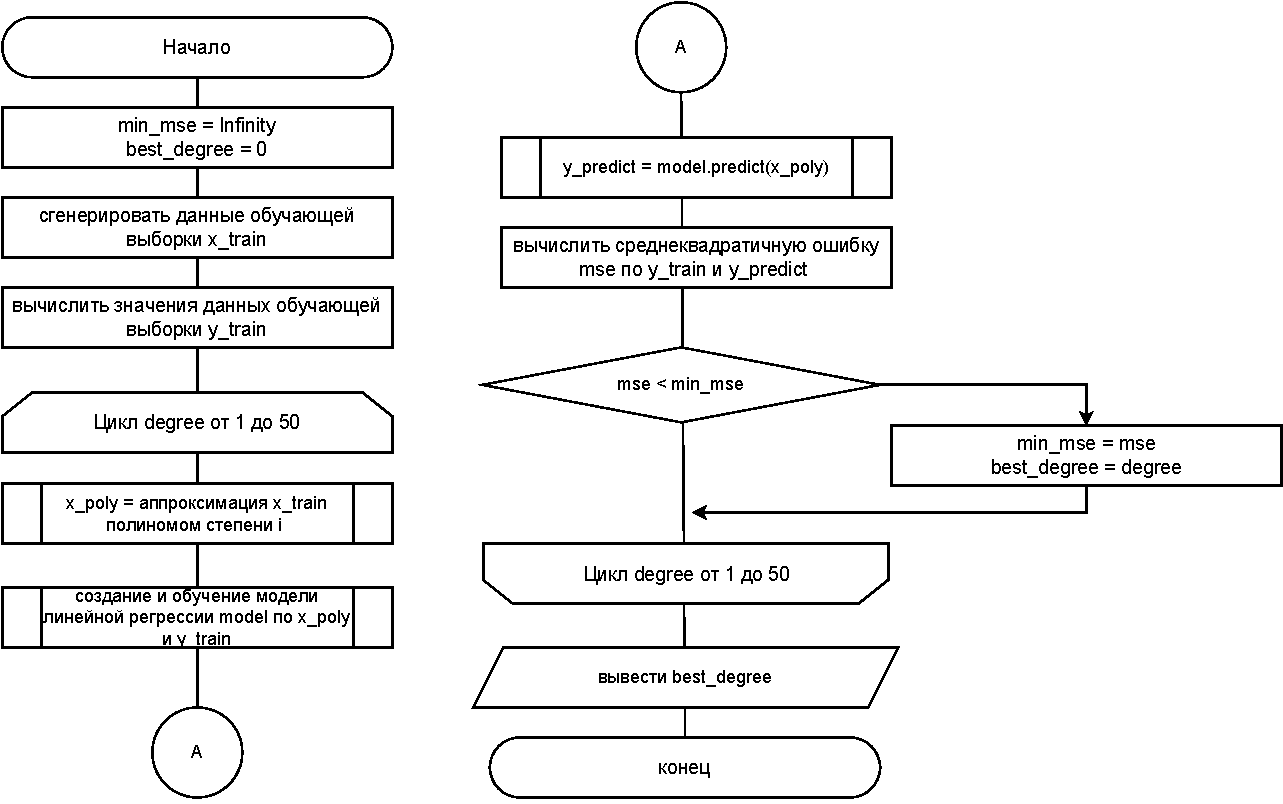
\includegraphics[width = \linewidth]{mml_lab_01.pdf}
  \caption{Схема работы алгоритма}
  \label{fig:algo_gen}
\end{figure}


\chapter{Практическая часть}

\section{Выбор средств разработки}
В качестве языка программирования был использован язык Python, поскольку этот язык кроссплатформенный и для него разработано огромное количество библиотек и модулей, решающих разнообразные задачи. 

В частности, имеются библиотеки, включающие в себя алгоритмы аппроксимации полиномом и линейной регрессии в библиотеке \cite{bib:sklearn}.

Для создания графиков была выбрана библиотека matplotlib \cite{bib:matplotlib}, доступная на языке Python, так как она предоставляет удобный интерфейс для работы с данными и их визуализации.

\section{Исследование ПО}

\subsection{Задача 1}
В листинге \ref{lst:gen} представлен код, вычисляющий оптимальную степень полинома по обучающей выборке и рисует зависимость среднеквадратичной ошибки модели по обучающей выборке от степени полинома.

\begin{lstlisting}[label=lst:gen,caption=код, решающий поставленную задачу]
import numpy as np
from sklearn.preprocessing import PolynomialFeatures
from sklearn.linear_model import LinearRegression
from sklearn.metrics import mean_squared_error
import matplotlib.pyplot as plt

theta_1 = 2
theta_2 = 1
theta_3 = 0.5

np.random.seed(0)
X_train = np.linspace(0, 10, 100)  
y_train = theta_1 * X_train + theta_2 * np.sin(X_train) + theta_3 + np.random.normal(0, 0.5, 100)  

min_mse = float('inf')
best_degree = 0
degrees = list(range(1, 50))
errors = []

for degree in degrees:
    poly_features = PolynomialFeatures(degree=degree)
    X_poly = poly_features.fit_transform(X_train.reshape(-1, 1))
    model = LinearRegression()
    model.fit(X_poly, y_train)

    y_pred = model.predict(X_poly)

    mse = mean_squared_error(y_train, y_pred)
    errors.append(mse)
    if mse < min_mse:
        min_mse = mse
        best_degree = degree

print(f"Optimal degree of poly: {best_degree}")

best_poly_features = PolynomialFeatures(degree=best_degree)
X_poly_best = best_poly_features.fit_transform(X_train.reshape(-1, 1))

best_model = LinearRegression()
best_model.fit(X_poly_best, y_train)

plt.plot(degrees, errors)
plt.xlabel('Degree of poly')
plt.ylabel('Value error')
plt.title('Dependence of value error on degree of poly')
plt.show()

\end{lstlisting}


На рисунке \ref{fig:points3} показана зависимость значения ошибки от степени полинома. Видно, что увеличение степени полинома необязательно даёт лучшие результаты в смысле уменьшения ошибки. 

\begin{figure}[h!]
  \centering
  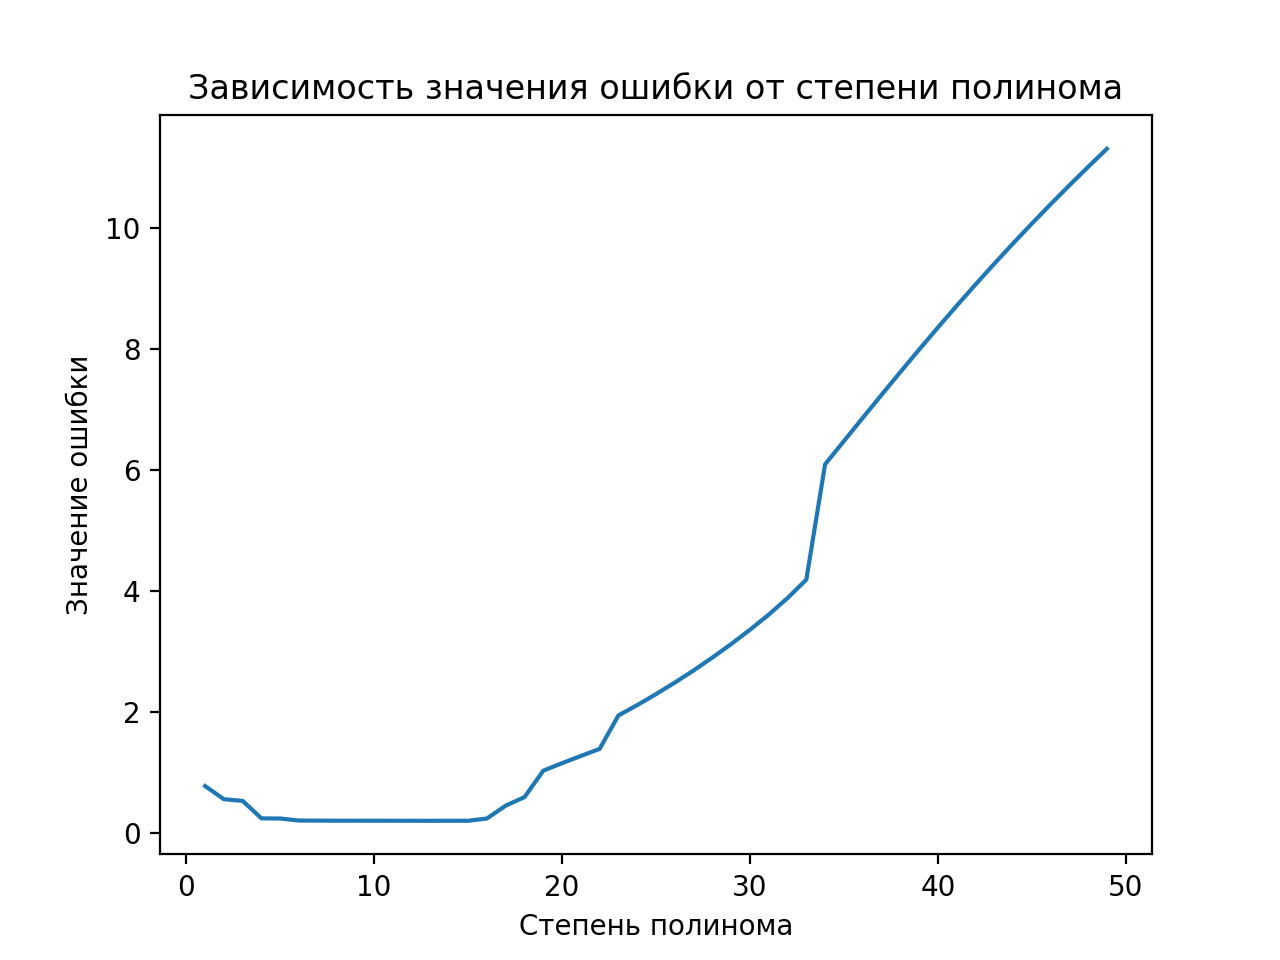
\includegraphics[width = \linewidth]{res.png}
  \caption{}
  \label{fig:points3}
\end{figure}
\newpage

Результат работы ПО -- было вычислено, что оптимальная степень полинома равна 13.

\newpage
\subsection{Задача 2}


В листинге \ref{lst:gen2} представлен код, вычисляющий оптимальную степень полинома по контрольной выборке и рисует зависимость среднеквадратичной ошибки модели (функционала эмпирического риска) для обучающей и контрольной выборок от степени полинома.

\begin{lstlisting}[label=lst:gen2,caption=код, решающий поставленную задачу]
import numpy as np
import matplotlib.pyplot as plt
from sklearn.preprocessing import PolynomialFeatures
from sklearn.linear_model import LinearRegression
from sklearn.metrics import mean_squared_error

def true_function(x):
    return 1 / (1 + 25 * x**2)

l = 21
X_train = np.array([4 * (i - 1) / (l - 1) - 2 for i in range(1, l + 1)]).reshape(-1, 1)
X_control = np.array([4 * (i - 0.5) / (l - 1) - 2 for i in range(1, l)]).reshape(-1, 1)
y_train = true_function(X_train)
y_control = true_function(X_control)

def fit_polynomial_regression(X, y, degree):
    poly_features = PolynomialFeatures(degree=degree)
    X_poly = poly_features.fit_transform(X)
    model = LinearRegression()
    model.fit(X_poly, y)
    return model, poly_features


def calculate_error(model, poly_features, X, y):
    X_poly = poly_features.transform(X)
    y_pred = model.predict(X_poly)
    return mean_squared_error(y, y_pred)


degrees = np.arange(1, 50)
train_errors = []
control_errors = []

for degree in degrees:
    model, poly_features = fit_polynomial_regression(X_train, y_train, degree)
    train_error = calculate_error(model, poly_features, X_train, y_train)
    control_error = calculate_error(model, poly_features, X_control, y_control)
    train_errors.append(train_error)
    control_errors.append(control_error)

plt.plot(degrees, train_errors, label='Train Error')
plt.plot(degrees, control_errors, label='Control Error')
plt.xlabel('Degree of Polynomial')
plt.ylabel('Mean Squared Error')
plt.title('Error vs Polynomial Degree')
plt.legend()
plt.show()


optimal_degree = degrees[np.argmin(control_errors)]
print(f'Optimal polynomial degree for approximation: {optimal_degree}')

\end{lstlisting}


На рисунке \ref{fig:points4} показана зависимость значения ошибки от степени полинома. Как и в предыдущей задаче, видно, что увеличение степени полинома необязательно даёт лучшие результаты в смысле уменьшения ошибки.

\begin{figure}[h!]
  \centering
  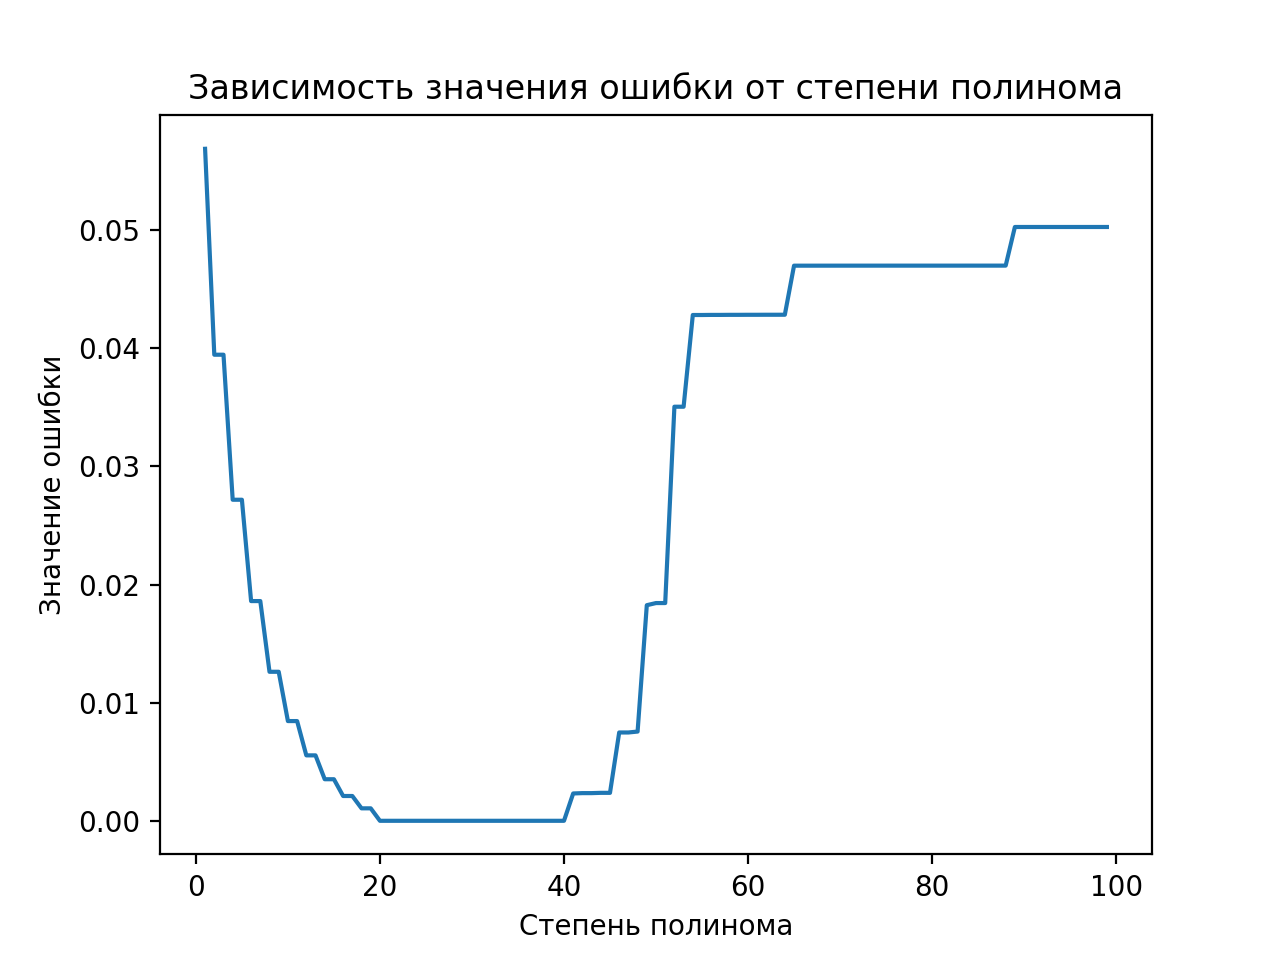
\includegraphics[width = \linewidth]{res_2_1.png}
  \caption{}
  \label{fig:points4}
\end{figure}

На рисунке \ref{fig:points5} показана зависимость значения ошибки от степени полинома для обучающей и контрольной выбоорок. Видим, что для контрольной выборки с определённого значения степени полинома ошибка стремительно растёт, что демонстрирует эффект Рунге -- эффект нежелательных осцилляций или колебаний вблизи крайних точек интерполяции при использовании полиномов высоких степеней.

\begin{figure}[h!]
  \centering
  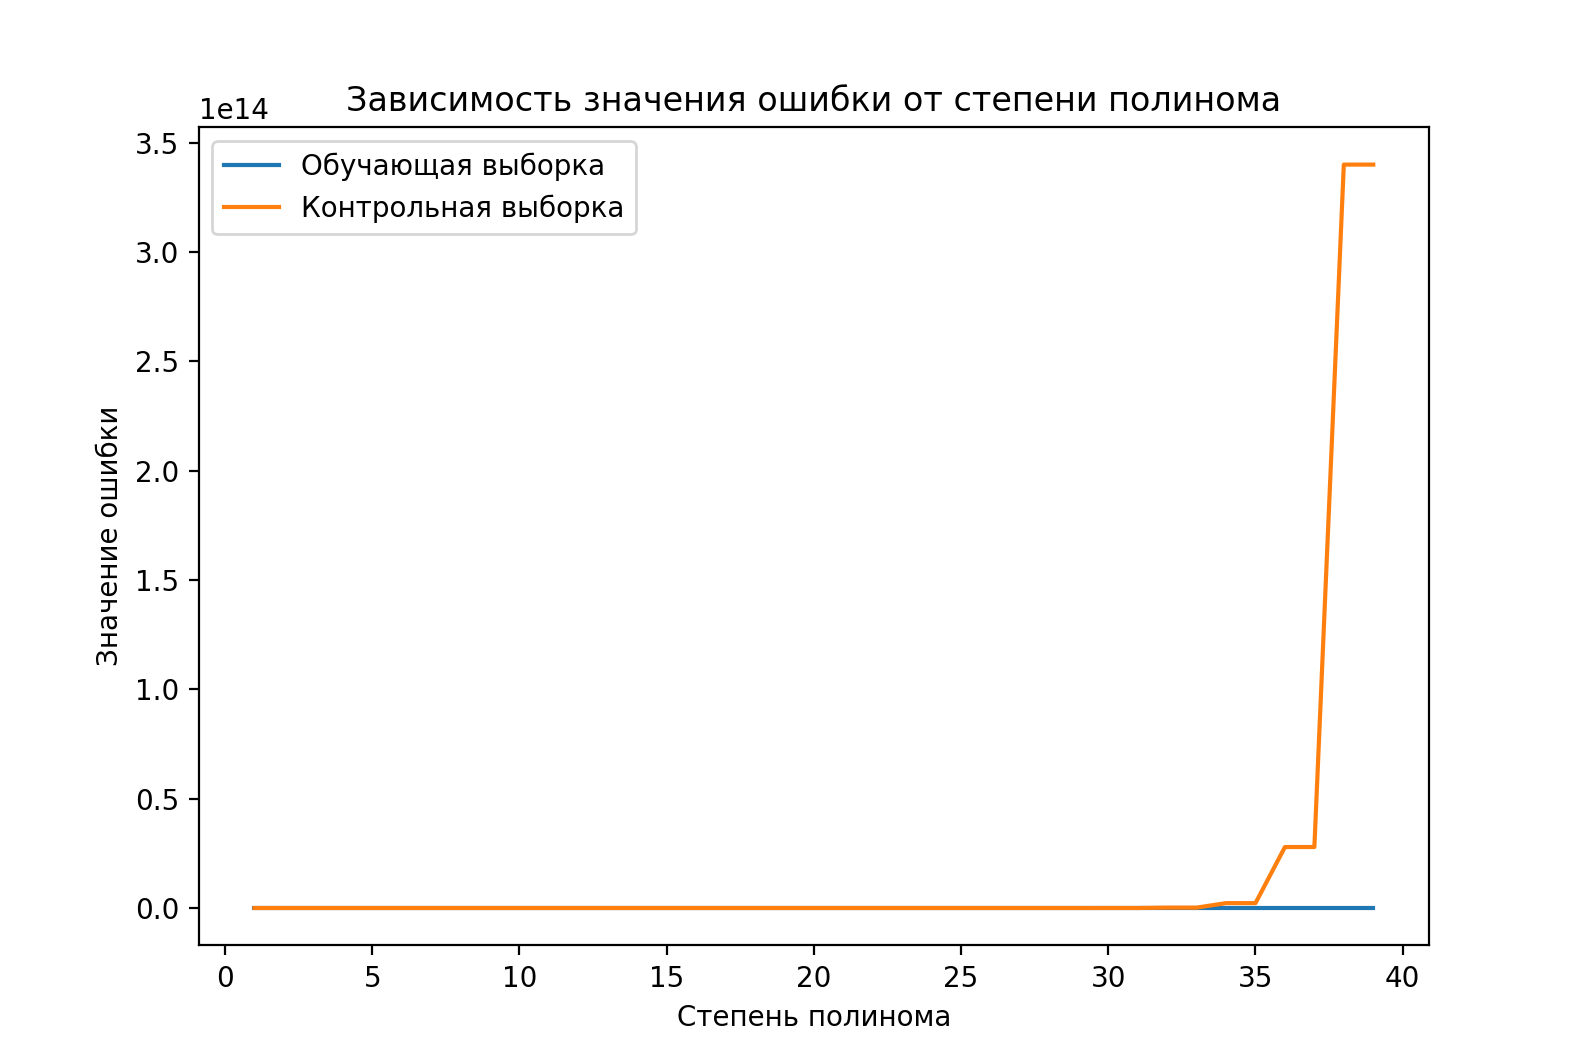
\includegraphics[width = \linewidth]{res_2_2.png}
  \caption{}
  \label{fig:points5}
\end{figure}
\newpage
Рассмотрим интервал низких степеней полинома для получения оптимальной степени полинома на рисунке \ref{fig:points6}.

\begin{figure}[h!]
  \centering
  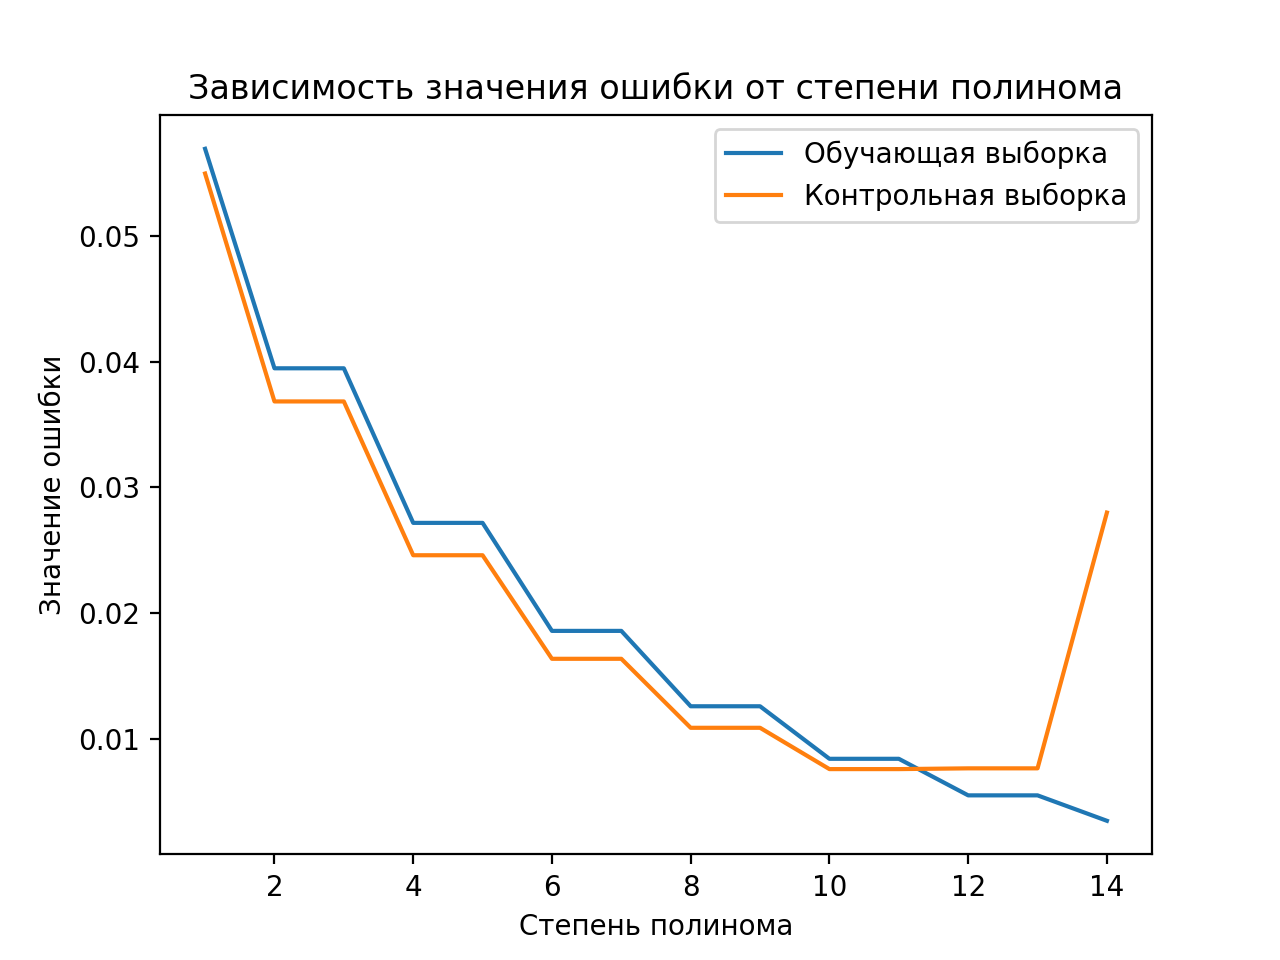
\includegraphics[width = \linewidth]{res_2_3.png}
  \caption{}
  \label{fig:points6}
\end{figure}


Видим, что оптимальная степень полинома равна 10.


\printbibliography[title={СПИСОК ИСПОЛЬЗОВАННЫХ\\ ИСТОЧНИКОВ}]
\addcontentsline{toc}{chapter}{СПИСОК ИСПОЛЬЗОВАННЫХ ИСТОЧНИКОВ}

\end{document}